\subsection{On J1331's central kinematics}

%==============
\begin{figure}
\centering
  \includegraphics[width=0.9\linewidth]{fig/B4_jam_profiles_errors_short_vcirc.ps}
  \caption{Comparison of the circular velocity curve of J1331's inner regions for different models: (a) JAM model with NFW DM halo from Section \ref{sec:results_JAM_NFW} and Figure \ref{fig:modelB4_models} (green). (b) Lens model from Section \ref{sec:results_lensing} and Figure \ref{fig:JAM_modelL} with $\alpha = 1.1$ (red dashed line), $\alpha = 1$ (red solid line) and $\alpha=0.9$ (red dash-dotted line). (c) Mass-follows-light model, which uses the F814W surface brightness in Table \ref{tab:MGEF814W} and the mass-to-light ratio in the Einstein radius, $\Upsilon^\text{ein}_\text{I,tot} = 5.56$, to generate a mass distribution, as in Figure \ref{fig:lenscomparelight} (orange line).  (d) Model from gas kinematics and Einstein mass found by \citet{SWELLSV} (their Figure 2, best model with 68\% confidence region) (blue lines).}
  \label{fig:vcirc_comparison}
\end{figure}
%==============

In Figure \ref{fig:vcirc_comparison} we compare the circular velocity curve found by \citet{SWELLSV} with a mass-follows-light model scaled to fit our Einstein mass (by multiplying the light distribution in Table \ref{tab:MGEF814W} with $\Upsilon_\text{I,tot}^\text{ein} = 5.56$). Within $R < 5''$ they agree with each other. 

The models in this work used more than just the Einstein mass to constrain the matter distribution at small radii: The lens mass model constrained also the shape of the mass distribution within the lensing image configuration at $R_\text{ein} \sim 1''$. The dynamical models used stellar kinematics inside $R' \simeq 3.5''$ \Wilma{[TO DO: Check]}. We compare the lens mass model's $v_\text{circ}$ (for $\alpha=1.0\pm 0.1$) with the NFW JAM model (Table \ref{tab:modelB4_bestfit}) in Figure \ref{fig:vcirc_comparison} as well. Within and around $R_\text{ein}$ they are consistent with each other, even though they where independently derived. They do not agree with the result by \citet{SWELLSV} and in Section \ref{sec:results_JAM_SB} we showed, that ``mass-follows-light'' is not a good model for J1331.

Overall, we were not able to find a consistent explanation for J1331's central $v_\text{rms}$ dip. It cannot be due to tangential velocity anisotropy in the center alone (see Section \ref{sec:results_JAM_SB}, Figure \ref{fig:JAM_modelA2}). It also cannot be explained by a strong contribution of DM inside the bulge together with a moderate tagential velocity anisotropy, because the corresponding DM halos would still be too massive to fit the data in the outer regions (see Section \ref{sec:results_JAM_NFW}, Figure \ref{fig:modelB4_vrms}]).e

Another feature in the stellar kinematics, that none of our JAM models was able to reproduce in the slightest and which we therefore excluded in the modelling, was the dip in $v_\text{rms}$ around $\sim 6''$, which occurs around the transition from bulge to disk (see Figures \ref{fig:F814W} and \ref{fig:kinematics}).